
\providecommand{\main}{..} 
\documentclass[\main/notes.tex]{subfiles} 

\begin{document} 
\begin{center} 
\textbf{{\Large Multi-Zone Milky Way Models}} 
\end{center} 

\noindent 
{\Large \textit{The Resultant [N/O]-[O/H] Relation}} 
\par\noindent 
Any viable model for nitrogen production in the Milky Way must accurately 
reproduce the observed abundances and their correlations with other elements. 
\textbf{Here we test a fiducial model for nitrogen yields.} 
The model has~$y_\text{N}^\text{CC} = 4.15\times10^{-4}$, 
$y_\text{N}^\text{Ia} = 0$, and~$y_\text{N}^\text{AGB}$ described by 
the~\citet{Cristallo2011} yields amplified by a factor of 5. 
Otherwise, the model is the same as the inside-out SFH model with diffusion 
migration from~\citet{Johnson2021}. 
Its predictions for the present day are shown in comparison to observational 
samples from a wide variety of astrophysical environments in 
Fig.~\ref{fig:no_oh_observed}. 
As discussed in~\citet{Vincenzo2016}, the observed [N/O]-[O/H] relation is more 
or less universal between systems; the comparison to the~\citet{Dopita2016} 
measurements further suggests that this extends to high redshift as well 
(z~$\sim$~3). 
It also appears to be relatively independent of the measurement method. 
\par 
For the fiducial model, each individual annulus at~$\rgal~\geq$ 2 kpc is 
represented by a point on the line. 
In general, it is more linear than the observed data. 
This suggests that at high metallicities, the model is under-predicting 
nitrogen production relative to oxygen, whereas it over-predicts it at low 
abundances. 
Since stellar migration only induces variability in~$\dot{Z}_\text{x}$ for some 
element~$x$ with delayed enrichment and only affects the time-averaged trend 
at large~\rgal~and early times, the late-time abundances should be reasonably 
described by the late-time equilibrium abundance of a one-zone model with 
similar parameters as one of the rings at a given~\rgal. 
Multiple studies focusing on the yields of AGB stars suggest that the nitrogen 
yields should depend more or less linearly on the initial mass of the 
progenitor~\citep{Cristallo2011, Ventura2013}, although the tables published 
by~\citet{Karakas2010} provide circumstantial evidence that they could be 
much higher for the most massive AGB stars, particularly at low metallicity. 
Since these studies largely agree on this qualitative result, the simplest 
way to recalibrate the yields is most likely by 
adjusting~$y_\text{N}^\text{CC}$ and its dependence on~$Z$, whose values span a 
much wider dynamic range between the~\citet{Limongi2018},~\citet{Sukhbold2018}, 
\citet*{Nomoto2013}, and~\citet{Woosley1995} results. 

\begin{figure*} 
\centering 
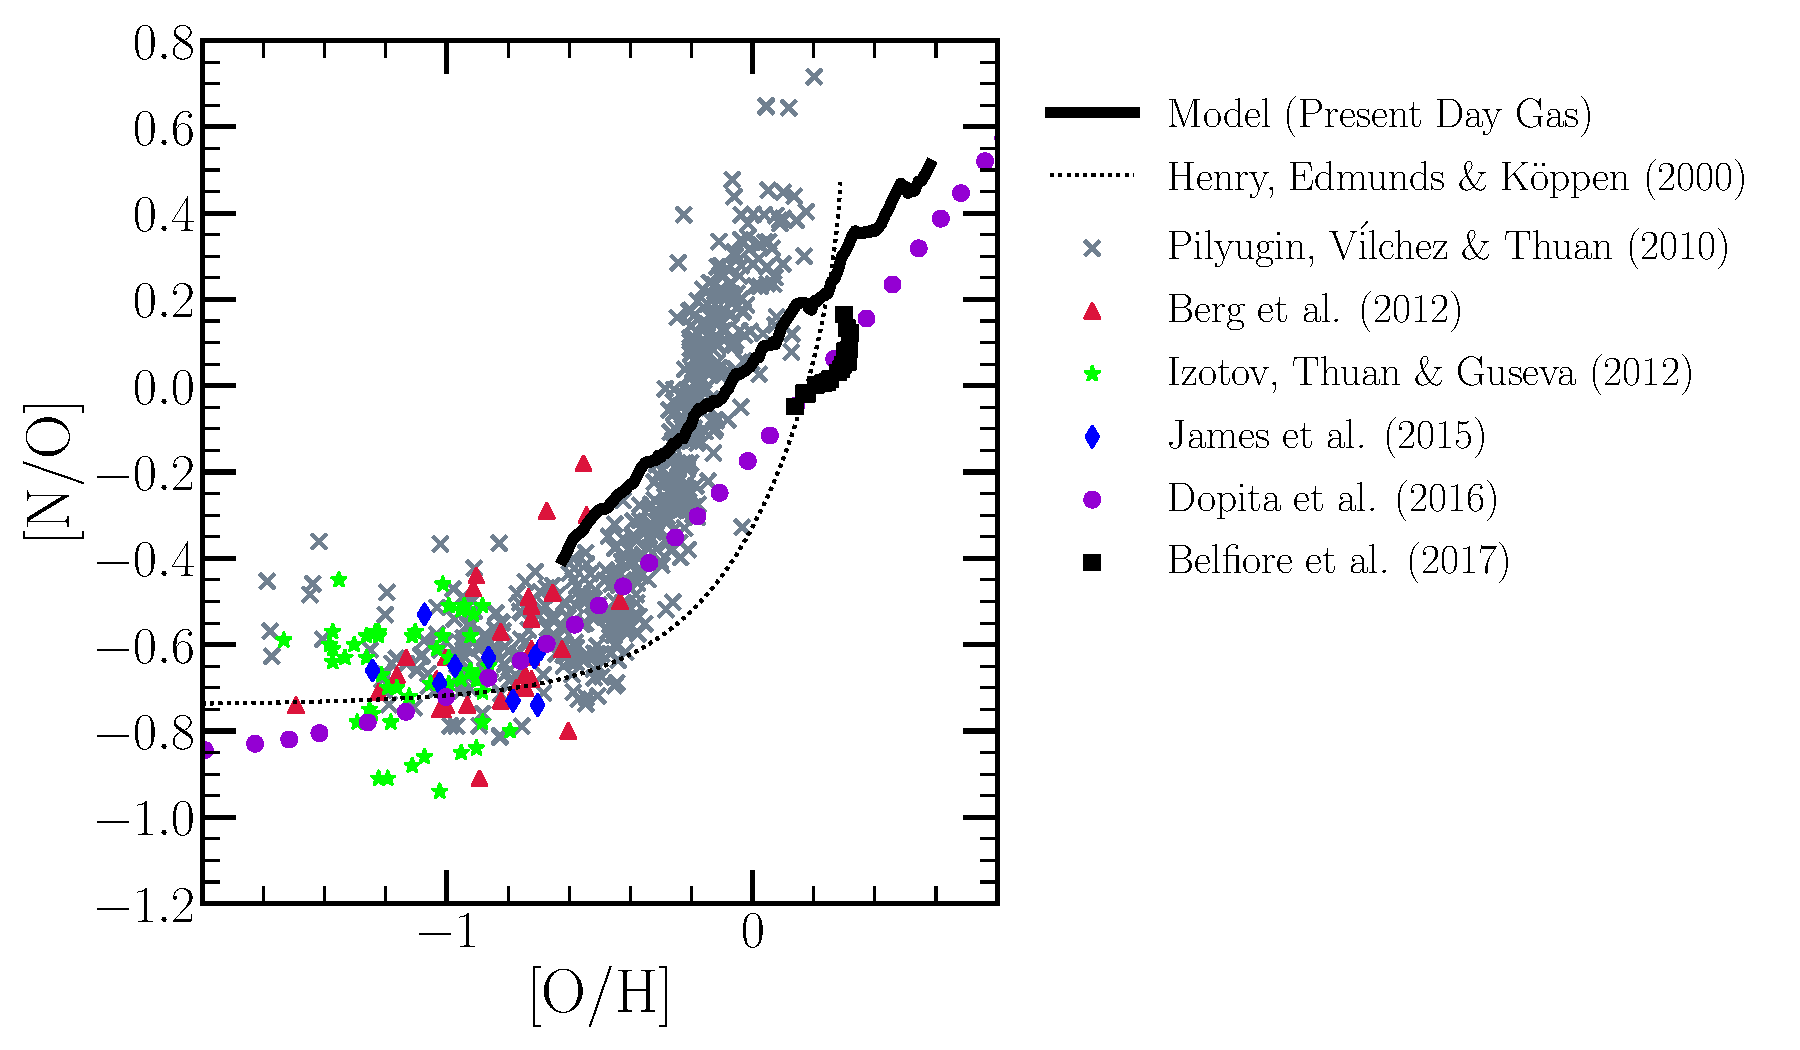
\includegraphics[scale = 0.5]{\main/multizone/no_oh_relation.pdf} 
\caption{
Observational results on the gas-phase [N/O]-[O/H] relation in comparison with 
a fiducial model at the present day (solid, thick black line). 
For the fiducial model, each individual ring at a radius of~$\rgal~\geq$ 2 kpc 
is plotted as a point on the line. 
The fit to an analytic chemical evolution model using data from Galactic HII 
regions, main sequence and halo stars, and damped lyman alpha systems 
from~\citet{Henry2000} is shown in a dotted black line. 
Abundances derived from electron temperatures of HII in nearby NGC spiral 
galaxies at shown in grey X's~\citep*{Pilyugin2010}. 
Measurements from blue, star forming diffuse dwarf galaxies probing the low 
metallicity regime are shown in red triangles~\citep{Berg2012}, green 
stars~\citep*{Izotov2012}, and blue diamonds~\citep{James2015}. 
Emission line measurements from high-redshift HII regions are shown in purple 
circles~\citep{Dopita2016}. 
A sample of star-forming galaxies from MaNGA are shown in black 
squares~\citep{Belfiore2017}. 
The~\citet*{Pilyugin2010},~\citet{Berg2012},~\citet*{Izotov2012}, 
and~\citet{James2015} measurements are for individual systems, while 
the~\citet{Dopita2016} and~\citet{Belfiore2017} data represent a 
population-averaged trend. 
Error bars are omitted for visual clarity. 
} 
\label{fig:no_oh_observed} 
\end{figure*} 

\textbf{Is the resultant [N/O]-[O/H] relation the result of the metallicity 
dependence of the yields only, or is the time-delay sufficiently important 
that it is instead a superposition of endpoints?} 
This question is addressed in Fig.~\ref{fig:no_oh_tracks}, which plots the 
present-day [N/O]-[O/H] relation in the gas-phase (parameterized by radius) 
as well as the evolutionary tracks (parameterized by time) for a selction of 
radii in the model. 
Since the evolutionary tracks show a noticeable dependence on~\rgal~at all 
times, it's quite clear from this that the time-dependence of AGB star 
nucleosynthesis is playing an important role in shaping the relation. 
The metallicity dependence is important as well, but this suggests that the 
time-dependence is strong enough that at least in this model,~\textbf{the 
[N/O]-[O/H] relation is arising out a superposition of endpoints}. 
This further suggests that these gas-phase abundance correlations should not be 
described by one-zone models reproducing the trend. 

\begin{figure*} 
\centering 
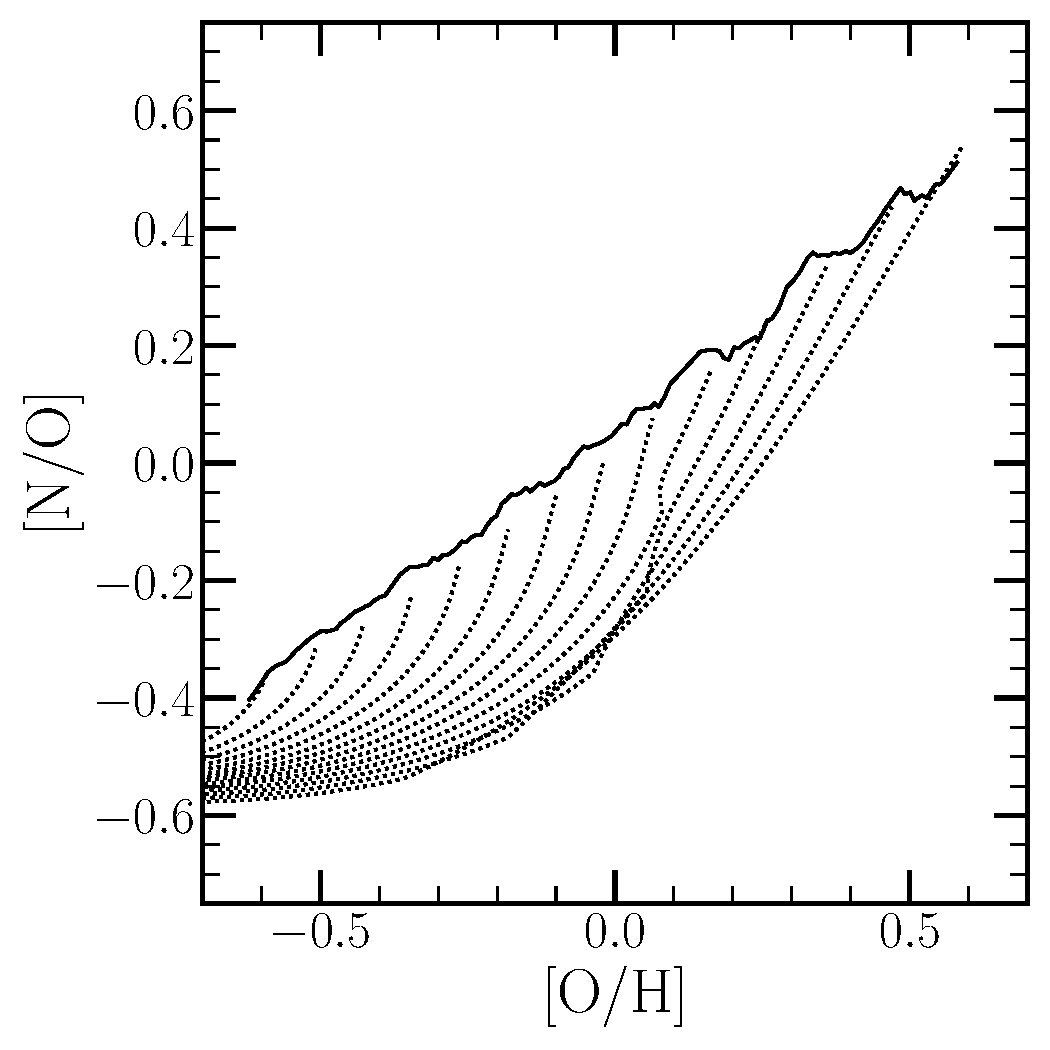
\includegraphics[scale = 0.5]{\main/multizone/no_oh_tracks.pdf} 
\caption{
The present-day gas-phase [N/O] relation as a function of [O/H] in the fiducial 
model for~$\rgal~\geq$ 2 kpc (solid), shown alongside the gas-phase 
evolutionary tracks (i.e. parameterized by time) for~\rgal~= 2, 3, 4, ... , 13, 
14, and 15 kpc rings. 
} 
\label{fig:no_oh_tracks} 
\end{figure*} 

\biblio 
\end{document} 
